\documentclass[border=6pt]{standalone}
\usepackage{tikz}
\usetikzlibrary{arrows.meta,positioning,calc,shapes.geometric,fit,backgrounds,patterns,matrix,decorations.pathreplacing}
\begin{document}
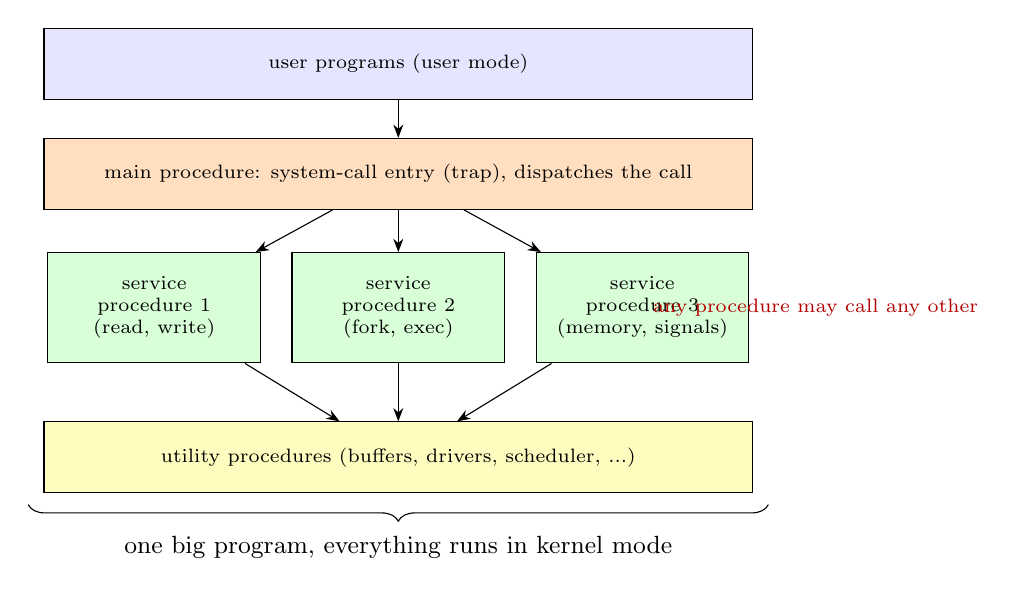
\begin{tikzpicture}[>=Stealth,font=\small]
\tikzstyle{b}=[draw,align=center,font=\scriptsize,minimum height=0.9cm]
\node[b,fill=blue!10,minimum width=9cm] (u) at (0,4) {user programs (user mode)};
\node[b,fill=orange!25,minimum width=9cm] (m) at (0,2.6) {main procedure: system-call entry (trap), dispatches the call};
\node[b,fill=green!15,minimum width=2.7cm,minimum height=1.4cm] (s1) at (-3.1,0.9) {service\\ procedure 1\\ (read, write)};
\node[b,fill=green!15,minimum width=2.7cm,minimum height=1.4cm] (s2) at (0,0.9) {service\\ procedure 2\\ (fork, exec)};
\node[b,fill=green!15,minimum width=2.7cm,minimum height=1.4cm] (s3) at (3.1,0.9) {service\\ procedure 3\\ (memory, signals)};
\node[b,fill=yellow!25,minimum width=9cm] (ut) at (0,-1.0) {utility procedures (buffers, drivers, scheduler, ...)};
\draw[->] (u) -- (m); \draw[->] (m) -- (s1); \draw[->] (m) -- (s2); \draw[->] (m) -- (s3);
\draw[->] (s1) -- (ut); \draw[->] (s2) -- (ut); \draw[->] (s3) -- (ut);
\node[font=\scriptsize,red!70!black] at (5.3,0.9) {any procedure may call any other};
\draw[decorate,decoration={brace,amplitude=6pt,mirror}] (-4.7,-1.6) -- (4.7,-1.6) node[midway,below=8pt,font=\small]{one big program, everything runs in kernel mode};
\end{tikzpicture}
\end{document}
